\subsection{Experiment~1: Mechanisms by which turnover influences equilibrium prevalence}
\label{ss:res-prevalence}
Figure~\ref{fig:prevalence} shows the trends in equilibrium STI prevalence  			
among the high, medium, low, risk groups, at different rates of turnover which 		%SM: suggest refer to Figure panels in text ".... the high (Figure 4a), medium (Figure 4b), ... etc. 
are depicted on the x-axis as
duration of time spent in the high risk group.
First, Figure~\ref{fig:prevalence} reveals an inverted U-shaped relationship
between STI prevalence and turnover in all three risk groups.
That is, equilibrium STI prevalence is higher in systems with slow turnover 
versus those with no turnover 
(region~A in Figure~\ref{fig:prevalence} ). Equilibrium STI prevalence then peaked						%SM: when talking about Region in the text, must refer to the figure.
at slightly faster turnover before declining in systems with even faster turnover 
(region~B in Figure~\ref{fig:prevalence} ).
Second, comparison of group-specific prevalence in Figure~\ref{fig:prevalence} shows that
the threshold turnover rate at which group-specific prevalence peaked
varied by risk group.
Prevalence in the high risk group peaked at the lower turnover threshold
(Figure~\ref{fig:prevalence-high}),
while prevalence in low risk group peaked at a higher turnover threshold								
(Figure~\ref{fig:prevalence-low}).

%SM: Figure 4 and Figure 5. (and appendix figures). suggest could make it more clear that 0.03 = no turnover in the caption. Figures should be stand-alone and 'no turnover' is not clear at all when reading those figures without the main text. 
%SM: Figure 7. Avoid asking reader (esp in the main text figures) to look at another figure (Figure 3) for the x-axis definition. Violates principe of stand-alone figures. Sometimes we have to do this (e.g. when pointing to an appendix, etc.) but in general - i think it will frustrate the reader to go back and forth to understand a figure on its own.

To explain the inverted U-shape and different turnover thresholds by group,							%SM: good. could follow this :). 
we examined the components contributing to prevalence,
first in the high risk group, and then in the low risk group.
\begin{figure}
\begin{minipage}[t]{0.475\linewidth}
  \centering
  \begin{subfigure}{0.85\linewidth}
    \centering
    \includegraphics[width=\linewidth]{{1d-prevalence-high-tau=0.1}.pdf}
    \caption{High risk}
    \label{fig:prevalence-high}
  \end{subfigure}\\
  \begin{subfigure}{0.85\linewidth}
    \centering
    \includegraphics[width=\linewidth]{{1d-prevalence-med-tau=0.1}.pdf}
    \caption{Medium risk}
    \label{fig:prevalence-med}
  \end{subfigure}\\
  \begin{subfigure}{0.85\linewidth}
    \centering
    \includegraphics[width=\linewidth]{{1d-prevalence-low-tau=0.1}.pdf}
    \caption{Low risk}
    \label{fig:prevalence-low}
  \end{subfigure}
  \caption{Relationship between equilibrium STI prevalence
    in high, medium, and low risk groups versus turnover rate.
    Regions A~and~B denote where equilibrium prevalence is increasing and decreasing
    with different rates of turnover, respectively.
    See Figure~\ref{fig:dur-group} for x-axis definition.}
  \label{fig:prevalence}
\end{minipage}\hspace{0.05\linewidth}%
\begin{minipage}[t]{0.475\linewidth}
  \centering
  \begin{subfigure}{0.85\linewidth}
    \centering
    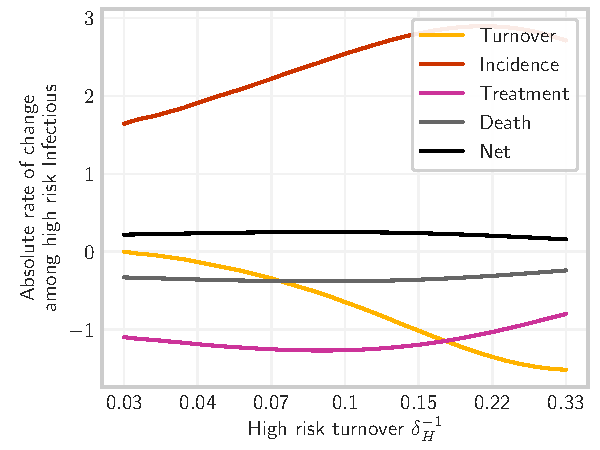
\includegraphics[width=\linewidth]{dX-abs-basic-high-I.pdf}
    \caption{High risk}
    \label{fig:dX-I-high}
  \end{subfigure}\\
  \begin{subfigure}{0.85\linewidth}
    \centering
    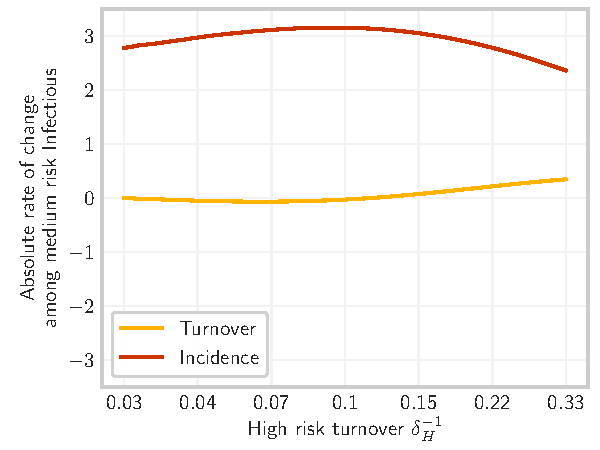
\includegraphics[width=\linewidth]{dX-abs-basic-med-I.pdf}
    \caption{Medium risk}
    \label{fig:dX-I-med}
  \end{subfigure}\\
  \begin{subfigure}{0.85\linewidth}
    \centering
    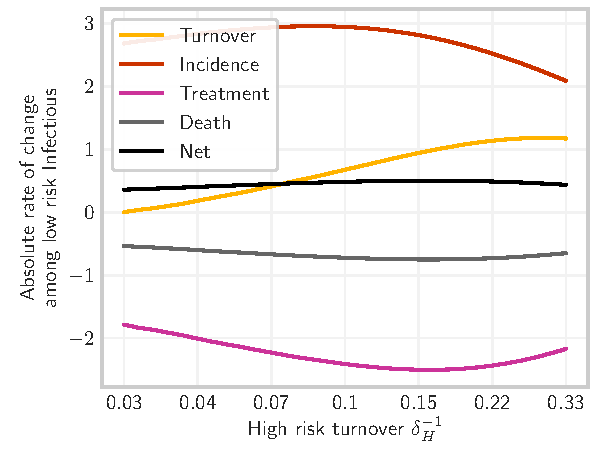
\includegraphics[width=\linewidth]{dX-abs-basic-low-I.pdf}
    \caption{Low risk}
    \label{fig:dX-I-low}
  \end{subfigure}\\
  \caption{Absolute rates of change at equilibrium
    (number of individuals gained/lost per year)
    among infectious individuals in each risk group,
    broken down by type of change:
    loss/gain via turnover, % ($+ \sum_j \phi_{ji} \mathcal{I}_j - \sum_j \phi_{ij} \mathcal{I}_i$),
    gain via incident infections, % ($+ \lambda_i \mathcal{S}_i$),
    loss via treatment, % ($- \tau \mathcal{I}_i$),
    loss via death, % ($- \mu \mathcal{I}_i$),
    and net change.
    Based on Eq.~(\ref{eq:model-I}).
    Rates of change do not sum to zero due to population growth.
    See Figure~\ref{fig:dur-group} for x-axis definition.}
  \label{fig:dX-I}
\end{minipage}
\end{figure}
\begin{figure}[!tbp]
  \centering
  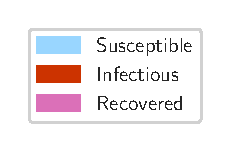
\includegraphics[width=0.6\linewidth]{flows-legend.pdf}\\
  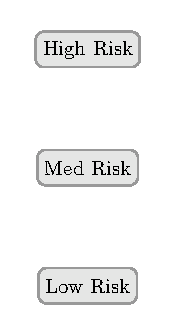
\includegraphics[width=0.11\linewidth]{flows-labels.pdf}
  \begin{subfigure}[t]{0.22\linewidth}
    \centering
    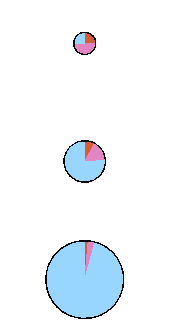
\includegraphics[width=\linewidth]{flows-none.pdf}
    \caption{No turnover}
    \footnotesize $\delta_H^{-1} = 0.062$
    \label{fig:flows-none}
  \end{subfigure}%
  \begin{subfigure}[t]{0.22\linewidth}
    \centering
    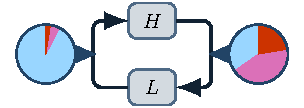
\includegraphics[width=\linewidth]{flows-low.pdf}
    \caption{Slow turnover}
    \footnotesize $\delta_H^{-1} = 0.062$
    \label{fig:flows-low}
  \end{subfigure}%
  \begin{subfigure}[t]{0.22\linewidth}
    \centering
    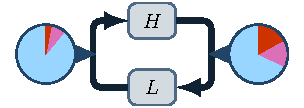
\includegraphics[width=\linewidth]{flows-high.pdf}
    \caption{Fast turnover}
    \footnotesize $\delta_H^{-1} = 0.062$
    \label{fig:flows-high}
  \end{subfigure}%
  \begin{subfigure}[t]{0.22\linewidth}
    \centering
    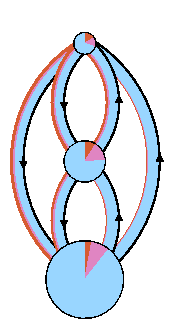
\includegraphics[width=\linewidth]{flows-extr.pdf}
    \caption{Very fast turnover}
    \footnotesize $\delta_H^{-1} = 0.062$
    \label{fig:flows-extr}
  \end{subfigure}\\[0.5em]
  $\null\hspace{0.11\linewidth}
  \underbrace{\hspace{0.44\linewidth}}_{\textrm{Region~A}}
  \underbrace{\hspace{0.44\linewidth}}_{\textrm{Region~B}}$
  \caption{Depiction of health states of individuals in each risk group		
    and of individuals moving between risk groups,
    obtained from models at equilibrium
    under four overall rates of turnover.
    Circle sizes are proportional to risk group sizes.
    Circle slices and arrow widths are also proportional to
    the proportion of health states within risk groups and
    among individuals moving between risk groups, respectively.
    However, circle sizes and arrow widths do not have comparable scales.}	%SM: tell reader that Appendix Figure 7 provides the numerical support for the proportions, etc.
  \label{fig:flows}
\end{figure}

\par
Figure~\ref{fig:dX-I} shows the four components which contributed to 
gain/loss of infectious individuals in each risk group:
1)~net gain/loss via turnover,
2)~gain via incident infections,
3)~loss via treatment, and
4)~loss via death,
for each risk group in the model,
at equilibrium under different rates of turnover.
Figure~\ref{fig:flows} also illustrates
the distribution of health states in each risk group
and among individuals moving between risk groups
under four different rates of turnover.
% --------------------------------------------------------------------------------------------------
\subsubsection{Influence of turnover on equilibrium prevalence in the high risk group}		%SM: becuase there are so many figures, i think will have to refer to the figure in almost every sentence. Before sending me the penulitmate version, please read out loud and check if any sentences seem unclear as to which figure they are referring to, etc.
\label{sss:res-prev-high}
As shown in Figure~\ref{fig:flows} at all four rates of turnover,
the proportion of individuals 
who were in the infectious state was largest in the high risk group. 
As infectious individuals left
the high risk group via turnover, they were largely 
replaced by susceptible individuals from lower risk groups (Figure C.7b). 			%SM: refer here to Figure 7b in Appendix so that the "numbers" can be corroborated.
For example, in the context of slow turnover (Figure 6b, Figure C.7b), 			%SM for each statement --> give clear example with numbers to support the statement.
X percent of individuals in the high risk group were in the infectious state,
and the absolute rate of change of the infectious state 
attributable to turnover was -XX (Figure C.7b) while the
absolute rate of change in the susceptible state attributable to 
turnover was +XX (Figure C.7a). The pattern of net loss of 
infectious individuals in the high risk group via turnover
persisted across the range of turnover rates (Figure~\ref{fig:dX-I-high}, yellow).			%SM: and Figure 7b?
This net loss of infectious individuals via turnover 
reduced STI prevalence within the high risk group (Figure XXX). 					%SM: insert right figure call out
At the same time, 
there was a net increase in susceptible individuals flowing into the high risk group
(Figure~\ref{fig:flows}) - the consequence of which was reduced protective herd effects
leading to a rise in incident infections among those at high risk when systems moved from 
no turnover to slow turnover (Figure~\ref{fig:dX-I-high}, red).
A third phenomena further mediated incidence reductions as systems
moved from no turnover to higher rates of turnover: 
the net movement of infectious individuals
from high to low risk (Figure~\ref{fig:flows}) reduced
the average number of partners per year on offer or available among 
individuals in the infectious state
(Figure~\ref{fig:C-I}). 
As shown in Appendix~\ref{aa:eqs-incidence},
modelled incidence in all risk groups was proportional to
the average number of partners per year among infectious individuals
(Figure~\ref{fig:C-I}),
and overall prevalence
(Figure~\ref{fig:prevalence-all}).
Thus, as the average number of partners per year among infectious individuals
fell with faster turnover, incidence decreased
(Figure~\ref{fig:incidence-all}).


\par
Therefore, the inverted U-shaped relationship between turnover rate
and equilibrium STI prevalence within the high risk group was mediated
by the above three phenomena acting in concert. When systems moved 
from no turnover to 
slow turnover, reduction in herd effects predominated leading to increasing
equilbrium prevalence in the presence of some turnover 
(region~A of Figure~\ref{fig:prevalence-high}).
When systems were modelled under faster and faster turnover,
removal of infectious individuals via turnover and changes in the characteristic of the 
sexual network (i.e. reduction in average number of partners per year among infectious individuals) 
predominated, leading to lower equlibrium prevalence
at faster rates of turnover (Figure~\ref{fig:prevalence-high}, region~B).
Accordingly, the inverted U-shaped relationship between turnover rate and equlibrium incidence 
followed a similar pattern within all three groups. 

% SM: did not understand the complex sentence below (sentence starting with "Moreover"). Not sure how it flowed nor what the main point was. suggest rephrase for clarity (?mutally enforcing exponential decline = wordy and unclear and makes reader feel dumb :) or remove or use suggested edits (but not sure if that is what you meant) = in sentence above.
%Moreover, as equilibrium incidence decreased across all groups
%with faster turnover for the same reason,
%equilibrium prevalence then decreased, which in turn reduced incidence,
%and so on in a mutually reinforcing exponential decline
(Figure~\ref{fig:prevalence}, region~B).
\begin{figure}
  \centering
  \begin{subfigure}[t]{0.32\linewidth}
    \centering
    \includegraphics[width=\linewidth]{{1d-C-I-tau=0.1}.pdf}
    \caption{Average number of partners per year among infectious individuals}
    \label{fig:C-I}
  \end{subfigure}%
  \begin{subfigure}[t]{0.32\linewidth}
    \centering
    \includegraphics[width=\linewidth]{{1d-prevalence-all-tau=0.1}.pdf}
    \caption{Overall prevalence}
    \label{fig:prevalence-all}
  \end{subfigure}%
  \begin{subfigure}[t]{0.32\linewidth}
    \centering
    \includegraphics[width=\linewidth]{{1d-incidence-all-tau=0.1}.pdf}
    \caption{Overall incidence}
    \label{fig:incidence-all}
  \end{subfigure}%
  \caption{Overall incidence and the non-constant factors of incidence versus turnover.
    The product of factors (\subref{fig:C-I}) and (\subref{fig:prevalence-all})
    is proportional to (\subref{fig:incidence-all}) overall incidence.
    See Appendix~\ref{aa:eqs-incidence} for proof.
    See Figure~\ref{fig:dur-group} for x-axis definition.}
  \label{fig:incidence-factors}
\end{figure}
% --------------------------------------------------------------------------------------------------
\subsubsection{Influence of turnover on equilibrium prevalence in the low risk group}
\label{sss:res-prev-low}
As shown in Figure~\ref{fig:flows}, at equilibrium, the low risk group was
composed mainly of susceptible individuals (e.g. X percent susceptible at slow turnover, Figure 5 and Figure C.7g).
Moving from a system without turnover to one 
with slow
turnover lead to a net influx of 
infectious (Figure Appendix C.7i) and treated (Figure C.7h) individuals and net removal of		%SM: Appendix Figure C.7 currently hides the curves with the legend. Grey and black a bit hard to differentiate; and same with red and pink. might make it harder on the reader. consider using dashed lines to differeniate similar colors, etc.
susceptible individuals (Figure C.7g). 		%SM: it is hard to see the decline in appendix figure C.7
The net influx of infectious individuals led to
higher equilibrium prevalence in the low risk group when the system
moved from no turnover to slow turnover
(Figure~\ref{fig:dX-I-low}, yellow).

%The net influx of treated individuals
%contributed to a small increase in herd immunity,
%but the herd immunity effect in the low risk group
%remained negligible due to
%the small proportion of treated relative to susceptible individuals. %SM: removed this sentence. I don't follow the logic. proportion "not susceptible" leads to herd effect. so the "due to..." part does not make sense to me the way currently written. If confusing me, may confuse others? So leave out as the statement also would require more 'evidence (i.e. show don't tell)' before it can be included as an explanation.

At the same time, incident
infections rose in the low risk group 
(Figure~\ref{fig:dX-I-low}, red) as the system moved from 
no turnover to slow turnover -
due to higher incidence in the total population (Figure~\ref{fig:incidence-all}) 
which was largely driven by  
reduced herd effects in the high risk group
(see Section~\ref{sss:res-prev-high}).

Thus, there were two phenomena working in concert
to increase equilibrium STI prevalence in the low risk group
at slow rates of turnover (Figure~\ref{fig:prevalence-low}, region~A).
\par
As systems moved to even faster turnover,
incident infections declined in 
the low risk group
(Figure~\ref{fig:dX-I-low}, red),		%SM: also refer to region B here?
due to lower incidence in the total population
(Figure~\ref{fig:incidence-all}) 
which was driven by 
decreasing number of partners per year among infectious individuals
(Figure~\ref{fig:C-I}).
The decline in incident infections in the low
risk group predominated over the influx
of infectious individuals from the medium and high risk groups
and equilibrium prevalence decreased in the low risk group when 
the system moved from slow to fast and very fast turnover
(Figure~\ref{fig:prevalence-low}, region~B).  %SM: and Figure 6 and Figure C.7 g,h,i?

Thus, there were three phenomena that
drove shifts in equilibrium prevalence in the low risk group 
at variable rates of turnover: changes in herd effects especially within the high risk group;
changes in characteristics of the sexual network; and influx of infectious individuals 
into the low risk group.

% --------------------------------------------------------------------------------------------------
\subsubsection{ Influence of turnover on ratio of STI prevalence ratio between high and low risk groups}
% JK: not really sure if this is the best title for this section.
As shown in Figure~\ref{fig:dX-I} (yellow lines), turnover created
a net loss of infectious individuals from the high risk group and
a net gain of infectious individuals in the low risk group.
In contrast, the influence of turnover on
the rate of incident infections followed a similar pattern			
in the high and low risk groups (Figure~\ref{fig:dX-I}, red).

As discussed above (specify where), as a system moves from
no turnover to faster turnover,
equilibrium prevalence
in the high risk group peaks and starts to fall while
equilibrium prevalence in the low risk group is still increasing (Figure 4a-c).
Even when equilibrium prevalence in the low risk group 
starts to fall at very fast turnover, it declines slower than
prevalence decline in the high risk group (Figure 4-c, region B).				%SM: correct? it looks like that from Figure 4a and 4c, but please confirm correct.
Thus, the ratio of equilibrium prevalence in the high risk
and low risk come closer to each other with 
faster turnover leading to a ``homogenizing effect'' of 
turnover on group-specific prevalence.% SM: I am ok with using term 'homogenizing' maybe once here, but perhaps not in discussion... really worried about how it might be stigmatizing if misunderstood...
That is, faster turnover minimizes risk heterogeneity as 
shown via the relationship between turnover and 
between-group STI prevalence ratios 
in Figure~\ref{fig:ratio-prevalence}
In particular, the prevalence ratio between highest and lowest risk groups
monotonically decreased with turnover
(Figure~\ref{fig:ratio-prevalence-high-low}).
% JK: I don't talk about prevalence ratios between high/med or med/low.
%     They're difficult to explain and I'm not sure it add anything,					
%     especially considering we haven't discussed the medium risk group
%     at all in this section...
%SM: Agree with the current approach to leave out. Though I have a feeling a reviewer will ask because it is shown in main text :). I agree would not explain now but move the prevalence ratio figures for medium: low and high:low to appendix since we are not talking about them here. They do not add but will distract the reader/reviewer. Also see my edits for the heading if we stick to comparing high vs. low for prevalence ratios as that is what we examine/vary for the  model fitting.

%SM: remove the sentences below....we may get asked to explain by reviewer more --> and if so, then will need to add more or explain this more clearly. I could not easily edit and do not think it adds enough at this stage since the 3 phenomena were already discussed in above sections. And so sentences below feel like they do not flow here.
%The homogenizing effect is also why, in the high risk group,
%lower rates of turnover were required
%to have a net decreasing effect on prevalence,
%as compared to in the low risk group.
%That is, the threshold rate of turnover at which
%prevalence in the high risk group peaked and then declined
%was lower than in the low risk group
%(Figure~\ref{fig:prevalence}).
\begin{figure}				%SM: move Figure 8b and 8c to appendix. Generally, try not to show figures / panels that are not discussed in main text. Most good jounrals/editors will ask to remove any figure panel not directly referred to in the main text at least once. i.e. since we do not refer to Figure 8b ever,...move to appendix.
  \centering
  \begin{subfigure}{0.31\linewidth}
    \centering\includegraphics[width=\linewidth]{{1d-ratio-prevalence-high-low-tau=0.1}.pdf}
    \caption{High vs Low risk}
    \label{fig:ratio-prevalence-high-low}
  \end{subfigure}
  \begin{subfigure}{0.31\linewidth}
    \centering\includegraphics[width=\linewidth]{{1d-ratio-prevalence-high-med-tau=0.1}.pdf}
    \caption{High vs Medium Risk}
    \label{fig:ratio-prevalence-high-med}
  \end{subfigure}
  \begin{subfigure}{0.31\linewidth}
    \centering\includegraphics[width=\linewidth]{{1d-ratio-prevalence-med-low-tau=0.1}.pdf}
    \caption{Medium vs Low Risk}
    \label{fig:ratio-prevalence-med-low}
  \end{subfigure}
  \caption{Equilibrium prevalence ratios between risk groups
    under different rates of turnover.
    See Figure~\ref{fig:dur-group} for x-axis definition.}
  \label{fig:ratio-prevalence}
\end{figure}
% ==================================================================================================
\subsection{Experiment~2: Inferred risk heterogeneity with vs without turnover}
\label{ss:res-infer}
Next, we compared the fitted parameters in models with versus without turnover
($\delta_H = 5$ vs $\delta_H = 33$ years).
Before model fitting, the predicted prevalence ratio
between high and low risk groups was lower with turnover versus without:
$\input{\datapath/values/turnover-prevalence-ratio-high-low.txt}$~vs~%
$\input{\datapath/values/no-turnover-prevalence-ratio-high-low.txt}$,
reflecting the homogenizing effect of turnover on group-specific prevalence
(Figure~\ref{fig:ratio-prevalence-high-low}).
Thus, when fitting the model to target prevalence values,
the fitted numbers of partners per year $C$ would have to compensate for
this difference in prevalence ratio with versus without turnover.
\par
After fitting the number of partners per year, both models predicted
the target equilibrium infection prevalence values of 20\%,~8.75\%,~3\%,~and~5\%
among the high, medium, low risk groups, and overall
(Figure~\ref{fig:tpaf-prevalence}).
However, in order to do so, the ratio of fitted partners
between high and low risk groups ($C_H~/~C_L$)
was higher with turnover than without:
$\input{\datapath/values/turnover-[fit]-C-ratio-high-low.txt}$~vs~%
$\input{\datapath/values/no-turnover-[fit]-C-ratio-high-low.txt}$
(Table~\ref{tab:fitting}).
That is, the inferred level of risk heterogeneity was higher
in the model with turnover than in the model without turnover.
In order to observe the same prevalence ratio in a system with turnover,
the homogenizing effect of turnover must be overcome by
greater heterogeneity in risk, as compared to a system without turnover.
\begin{table}
  \centering
  \caption{Equilibrium partnership formation rates and prevalence
    among the high and low risk groups
    predicted by the models with and without turnover,
    before and after model fitting.}
  \label{tab:fitting}
  \begin{tabularx}{0.7\linewidth}{r *{6}{Y}}
	\toprule
  Model & $C_H$ & $C_L$ & $C_H~/~C_L$ & $P_H$ & $P_L$ & $P_H~/~P_L$\\\midrule
  Base &
    \input{\datapath/fit/Base-C-high.txt}
  & \input{\datapath/fit/Base-C-low.txt}
  & \input{\datapath/fit/Base-C-ratio.txt}
  & \input{\datapath/fit/Base-prevalence-high.txt}
  & \input{\datapath/fit/Base-prevalence-low.txt}
  & \textbf{\input{\datapath/fit/Base-prevalence-ratio.txt}}\\
  V3 &
    \input{\datapath/fit/V3-C-high.txt}
  & \input{\datapath/fit/V3-C-low.txt}
  & \input{\datapath/fit/V3-C-ratio.txt}
  & \input{\datapath/fit/V3-prevalence-high.txt}
  & \input{\datapath/fit/V3-prevalence-low.txt}
  & \textbf{\input{\datapath/fit/V3-prevalence-ratio.txt}}\\
  Base [fit] &
    \input{\datapath/fit/Base-fit-C-high.txt}
  & \input{\datapath/fit/Base-fit-C-low.txt}
  & \textbf{\input{\datapath/fit/Base-fit-C-ratio.txt}}
  & \input{\datapath/fit/Base-fit-prevalence-high.txt}
  & \input{\datapath/fit/Base-fit-prevalence-low.txt}
  & \input{\datapath/fit/Base-fit-prevalence-ratio.txt}\\
  V3 [fit] &
    \input{\datapath/fit/V3-fit-C-high.txt}
  & \input{\datapath/fit/V3-fit-C-low.txt}
  & \textbf{\input{\datapath/fit/V3-fit-C-ratio.txt}}
  & \input{\datapath/fit/V3-fit-prevalence-high.txt}
  & \input{\datapath/fit/V3-fit-prevalence-low.txt}
  & \input{\datapath/fit/V3-fit-prevalence-ratio.txt}\\
  \bottomrule
\end{tabularx}
\end{table}
% ==================================================================================================
\subsection{Experiment~3: Influence of turnover on the tPAF of the high risk group}
\label{ss:res-tpaf}
Finally, we compared the predicted tPAF of the high risk group
with and without turnover, after fitting to the same prevalence data
(Figure~\ref{fig:tpaf-fit}).
The tPAF approaches 1 for both models over the 50 year period,
indicating that unmet treatment needs of the high risk group
are central to epidemic persistence in both scenarios.
% SB: Crucial.
The estimated tPAF of the high risk group is also higher
in the model with turnover versus
in the model without turnover
over all time horizons,
implying that models which fail to capture turnover dynamics which are present in reality
may underestimate the tPAF of high risk groups.
This increase in tPAF of the high risk group can be attributed to
a higher ratio of fitted partners $C_H~/~C_L$
in the model with turnover is higher than in the model without
(Experiment~2).
The increased partner ratio affords
a higher risk of onward transmission to the high risk group
in the model with turnover, and thus an increase in tPAF.
\begin{figure}[!tbp]
  \centering
  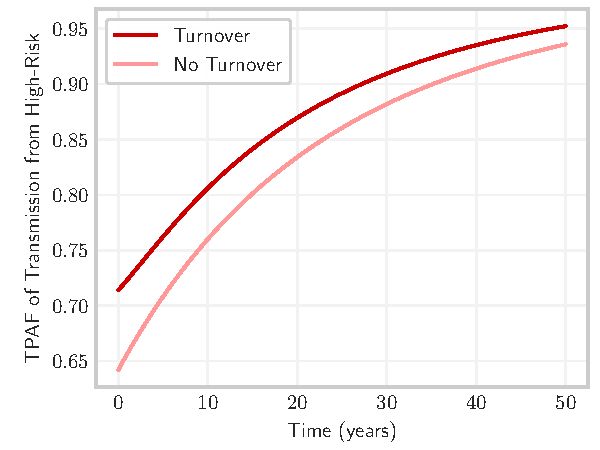
\includegraphics[width=0.5\linewidth]{sit-tpaf-tpaf-high-all-vs=fit.pdf}
  \caption{Transmission population attributable fraction (tPAF)
    of the high risk group in models with and without turnover,
    after fitting the number of partners per year to group-specific prevalence.}
  \label{fig:tpaf-fit}
\end{figure}
% LW: I think this is the key message and valid.
% SS: This section perhaps could be a bit clearer as clearly very important
%     Is there a way to more explicitly talk about new infections
%     in the low / medium risks coming from prevalent infections
%     entering into these states from high risk groups and that
%     subsequent infections emanating from these individuals are thus still
%     linked back to prior history in the high risk group?
% JK: Great point and I realized this was not emphasized anywhere in the paper.
%     However, I think this section is not the right place for it,
%     as the increase in TPAF is really attributable to the higher estimated
%     partners ratio from Experiment 2.
%     However, I highlight that infections in low risk groups can originate
%     from higher risk period in the discussion,
%     since it kind of gets lost in Experiment 1.
